\section{Methodology}
\label{sec:methodology}

\subsection{Window Slicing}

We use a window-slicing backtest with a 10-year training window and a 1-year test window. Over the 2006--2023 evaluation period, this yields 18 annual test slices. For each annual test slice, all model components are re-estimated using only past data. This includes the predictive regression and, when needed, the stock-to-ETF relatedness structure. In contrast to a single expanding fit, this design keeps the learning problem local in time and allows the available stock universe to evolve from window to window.

\begin{figure}[H]
\centering
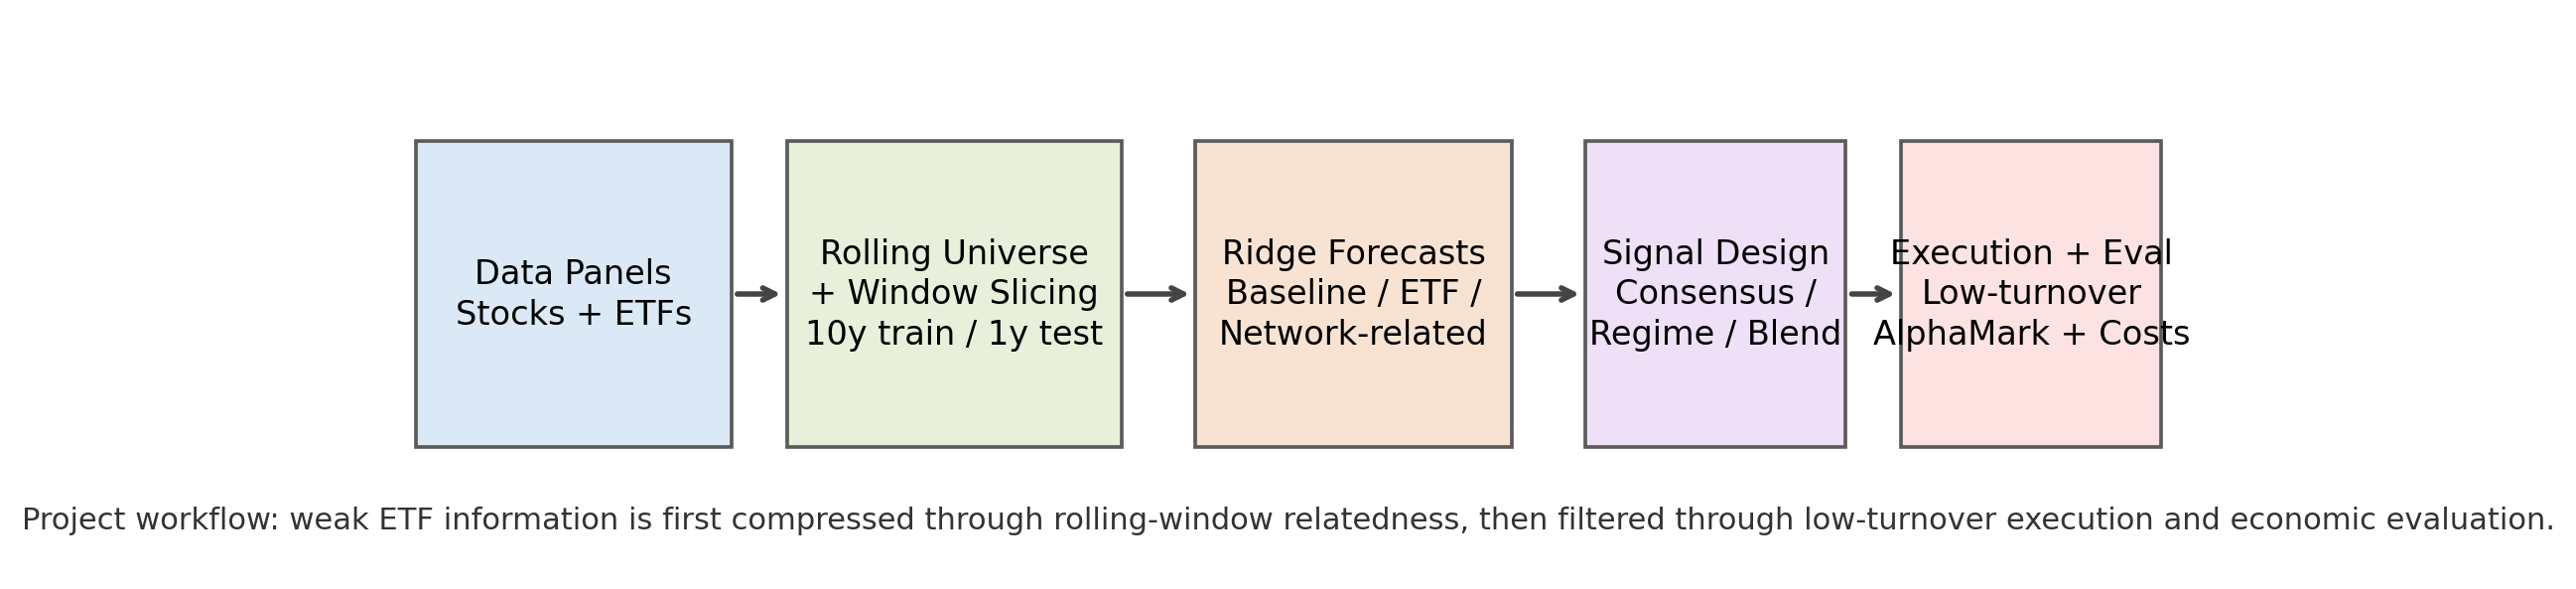
\includegraphics[width=\linewidth]{figures/pipeline_schematic.png}
\caption{Project workflow. ETF information is first summarized through rolling-window relatedness and then passed through explicit holding-period and rebalance rules before economic evaluation.}
\label{fig:pipeline}
\end{figure}

\subsection{Rolling-Universe Eligibility}

The stock universe is dynamic. For a stock to enter a given model in a given window, it must have the features and target required by that specific model inside the local train-test split. This detail matters because the eligible universe is not the same across the baseline, raw ETF, and network-style models. The resulting design is therefore both rolling in time and model-dependent in coverage.

\subsection{Ridge Regression and Feature Design}

All predictive models are estimated with Ridge regression. The initial model family includes:
\begin{itemize}[leftmargin=1.4em]
  \item a stock-only HAR baseline,
  \item a raw ETF model with a large ETF feature block,
  \item a network-style model using ETF-linked neighbor structure.
\end{itemize}

The stock-only HAR baseline has the form
\[
\hat r^{\mathrm{base}}_{i,t+1}
=
\beta_0+\beta_d r^{(d)}_{i,t}+\beta_w r^{(w)}_{i,t}+\beta_m r^{(m)}_{i,t}.
\]
The raw ETF model augments the baseline with a large set of daily ETF covariates available in the current window. The network-style model augments the baseline with a single neighbor-lag feature built from ETF-related stock similarity.

The raw ETF experiment is informative precisely because it fails: naive high-dimensional ETF expansion proves unstable and economically unconvincing. That result motivates the later stock-specific ETF summaries.

\subsection{Top-1 and Top-3 ETF Compression}

To reduce dimensionality, we summarize ETF information at the stock level through local relatedness. Let $\mathrm{Top1}(i)$ denote the ETF most related to stock $i$ within the current training window, and let $\mathrm{Top3}(i)$ denote the three most related ETFs. We then construct:
\[
\hat r^{\mathrm{top1}}_{i,t+1}
=
\hat r^{\mathrm{base}}_{i,t+1}
+ \gamma \, ETF^{\mathrm{Top1}(i)}_{d,t},
\]
\[
\hat r^{\mathrm{top3}}_{i,t+1}
=
\hat r^{\mathrm{base}}_{i,t+1}
+ \gamma \cdot \frac{1}{3}\sum_{e \in \mathrm{Top3}(i)} ETF_{e,d,t}.
\]

These ETF summaries are low-dimensional by construction and are much easier to interpret economically than a large raw ETF block.

\subsection{Network Feature Construction}

For the network-style models, we first construct a stock--ETF relatedness matrix inside the training window. This matrix is then converted into a stock--stock neighbor graph by comparing stocks through their ETF exposure patterns. For each stock, we keep the top-5 neighbors and define a lagged neighbor-return feature
\[
\mathrm{feat}^{\mathrm{nbr}}_{i,t}
=
\sum_{j \in \mathcal{N}_5(i)} w_{ij} r_{j,t},
\]
where the weights $w_{ij}$ are normalized across the selected neighbors. This feature is meant to capture peer effects implied by similarity in ETF linkage. In practice, however, the network-based specifications were not strong enough to become our final strategy family.

\subsection{Execution Layer}

Predicted signals are mapped to long-short portfolios. Let $s_{i,t}$ denote the selected strategy signal and let $\mathrm{bet\_size}_{i,t}$ denote either equal-weight sizing or lagged market-cap sizing. Daily portfolio weights are normalized as
\[
w_{i,t}
\propto
\mathrm{sign}(s_{i,t}) \cdot |\mathrm{bet\_size}_{i,t}|,
\qquad
\sum_i |w_{i,t}| = 1.
\]

The execution layer includes two turnover controls:
\begin{itemize}[leftmargin=1.4em]
  \item \texttt{hold\_days}: the minimum time before another rebalance is allowed;
  \item \texttt{rebalance\_threshold}: the minimum change between the current and target portfolios required to trigger a rebalance.
\end{itemize}

The target portfolio is only implemented if enough time has passed since the last rebalance and the desired portfolio differs sufficiently from the currently held one. This execution rule is central to the final results. Several signals that look attractive on a gross basis deteriorate quickly under costs when rebalanced too frequently, but remain viable under slower trading schedules.

\subsection{AlphaMark and Cost Sensitivity}

We use AlphaMark as the main standardized gross-performance evaluation tool. In the updated version of the project, AlphaMark is run with multiple quantile slices (\texttt{qr\_100}, \texttt{qr\_75}, \texttt{qr\_50}, and \texttt{qr\_25}) so that we can study whether the strongest performance appears in the full universe or in more selective parts of the signal ranking.

In addition, we run a separate tradability review under 10, 20, and 50 basis point cost assumptions. These basis-point costs should be interpreted as simplified all-in trading-cost scenarios that proxy for commissions, fees, spread, slippage, and market impact, applied proportionally to turnover:
\[
\mathrm{net\ return}_t
=
\mathrm{gross\ return}_t
-
\mathrm{turnover}_t \times c.
\]

This dual evaluation framework is deliberate. AlphaMark tells us whether the signal is economically meaningful on a gross basis, while the cost review tells us whether that apparent alpha survives a basic implementation test.
